\subsection{Filterspezifikation}

Beim zu realisierenden Stubfilter handelt es sich um ein Tiefpass-Filter 5. Ordnung, mit einer Grenzfrequenz (Passband) $f_C = 0.8GHz $ und einer Bezugsfrequenz $f_{\frac{\lambda}{4}} = 2GHz$. Die Bezugsfrequenz $f_{\frac{\lambda}{4}}$ definiert die Länge l der gleich langen Leitungsstücke uns ist folglich:

\begin{equation*}
l = \frac{\lambda}{4} = \frac{c}{4 \cdot f} = \frac{300\cdot 10^6 \lbrack\frac{m}{s}\rbrack}{4 \cdot 2 \lbrack GHz \rbrack} =37.5 \lbrack mm \rbrack
\end{equation*}

Zudem wird das Stubfilter von einem Prototypfilter (Tiefpass 5. Ordnung) 
mit den Elementwerte $g_0$ bis $g_6$ abgeleitet.

\begin{figure}[h!]
\centering
 	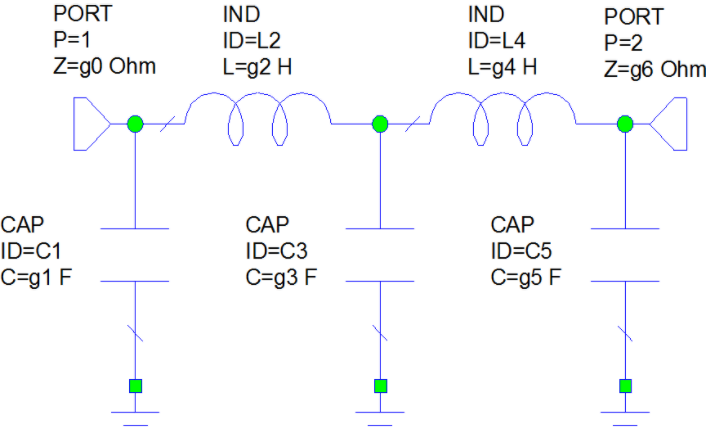
\includegraphics[width=\imagewidth]{images/Topologie_Prototyp.png}
 	\caption{Topologie des Prototypfilters}
 	\label{fig:Topologie_Prototyp.png}
\end{figure}

\begin{mdframed}
\begin{equation*} 
\begin{array}{rclcl} 
g_0 & = & 1 \\ 
g_1 & = & 0.973 \\ 
g_2 & = & 1.372 \\ 
g_3 & = & 1.803 \\ 
g_4 & = & 1.372 \\ 
g_5 & = & 0.973 \\ 
g_6 & = & 1 \\ 
\end{array} 
\end{equation*} 
\end{mdframed}

Durch Betrachtung der g-Parameter kann nicht direkt darauf geschlossen werden, um welchen Filtertyp (Chebyshev, Butterworth, Elliptic) es sich handelt. Deshalb wurde eine Simulation in Mirowave Office (MWO) durchgeführt. Diese zeigt, dass es sich beim Prototypfilter um ein Chebyshev Filter des Typs 1 handelt. Typisch für ein solches Chebyshev Filter ist ein Equirippel im Passband während im Stopband kein Rippel auszumachen ist. 

Die Übersichtsdarstellung der Eingügedämpfung S21 (Abb. \ref{fig:Ovw_Prototyp}) zeigt, dass das Filter keinen Stopbandrippel aufweist.

\begin{figure}[h!]
\centering
 	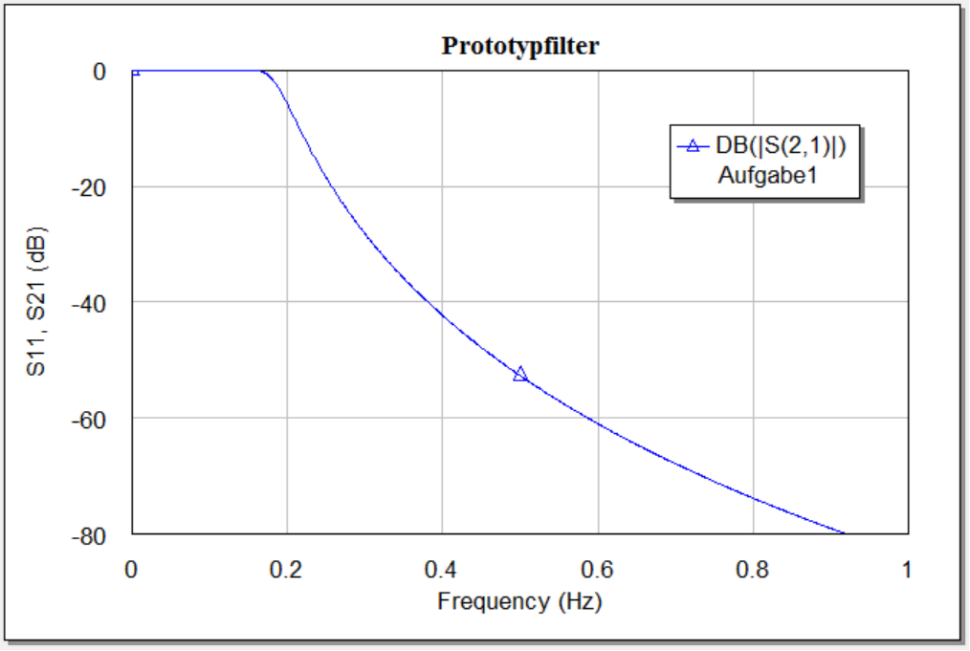
\includegraphics[width=\imagewidth]{images/Ovw_Prototyp.png}
 	\caption{Übersichtsdarstellung des Prototypfilters}
 	\label{fig:Ovw_Prototyp}
\end{figure}

Während die Detailanssicht der Einfügedämpfung S21 in Abb. \ref{fig:Prototyp_Passbandrippel} den kleinen Equirippel des Passbands sichtbar macht. Ausserdem zeigt sich aus der Detailansicht, dass das Filter wie erwartete eine Grenzfrequenz von $\omega_C = 1$ aufweist.

\begin{mdframed}
\begin{equation*} 
\begin{array}{rclcl} 
Equirippel & = & -0.04355 dB \\ 
\omega_C & = & 1 \\ 
f_C & = & 0.1592 Hz \\ 
\end{array} 
\end{equation*} 
\end{mdframed}

\begin{figure}[h!]
\centering
 	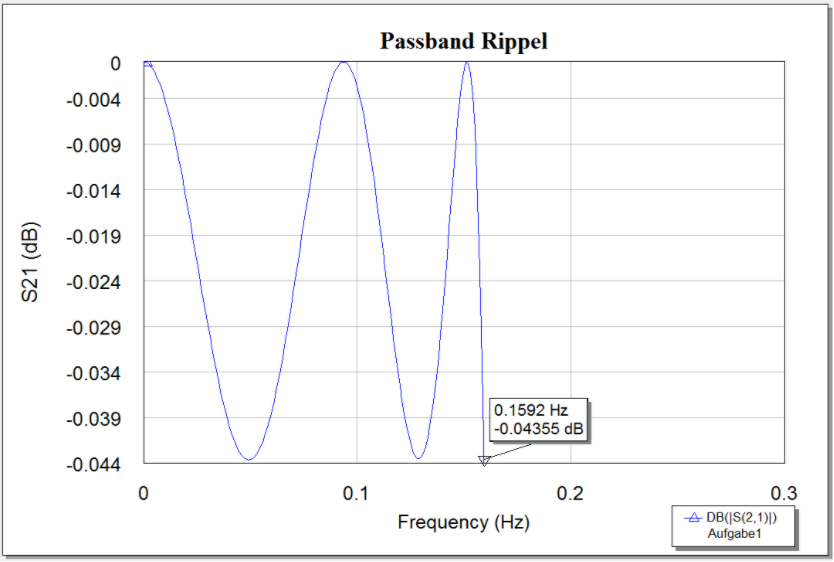
\includegraphics[width=\imagewidth]{images/Prototyp_Passbandrippel.png}
 	\caption{Equirippel im Passband}
 	\label{fig:Prototyp_Passbandrippel}
\end{figure}

Ein verlustloses Filter lässt sich nicht nur mit der Einfgedämpfung S21 sondern auch mit der Reflexion S11 beschreiben, weil der folgende Zusammenhang gilt:

\begin{equation}
{|S11|}^2 + {|S21|}^2 = 1
\end{equation}

Somit kann die Reflexion im Passband mithilfe des Equirippels im Passband berechnet werden.

\begin{equation}
|S11| = \sqrt{1-{|Equirippel|}^2} = -20 dB
\end{equation}

Um das Resultat zu validieren, wurde die Reflexion S11 des Filter simuliert und in Abb. \ref{fig:Prototyp_Reflexion} dargestellt.

\begin{figure}[h!]
\centering
 	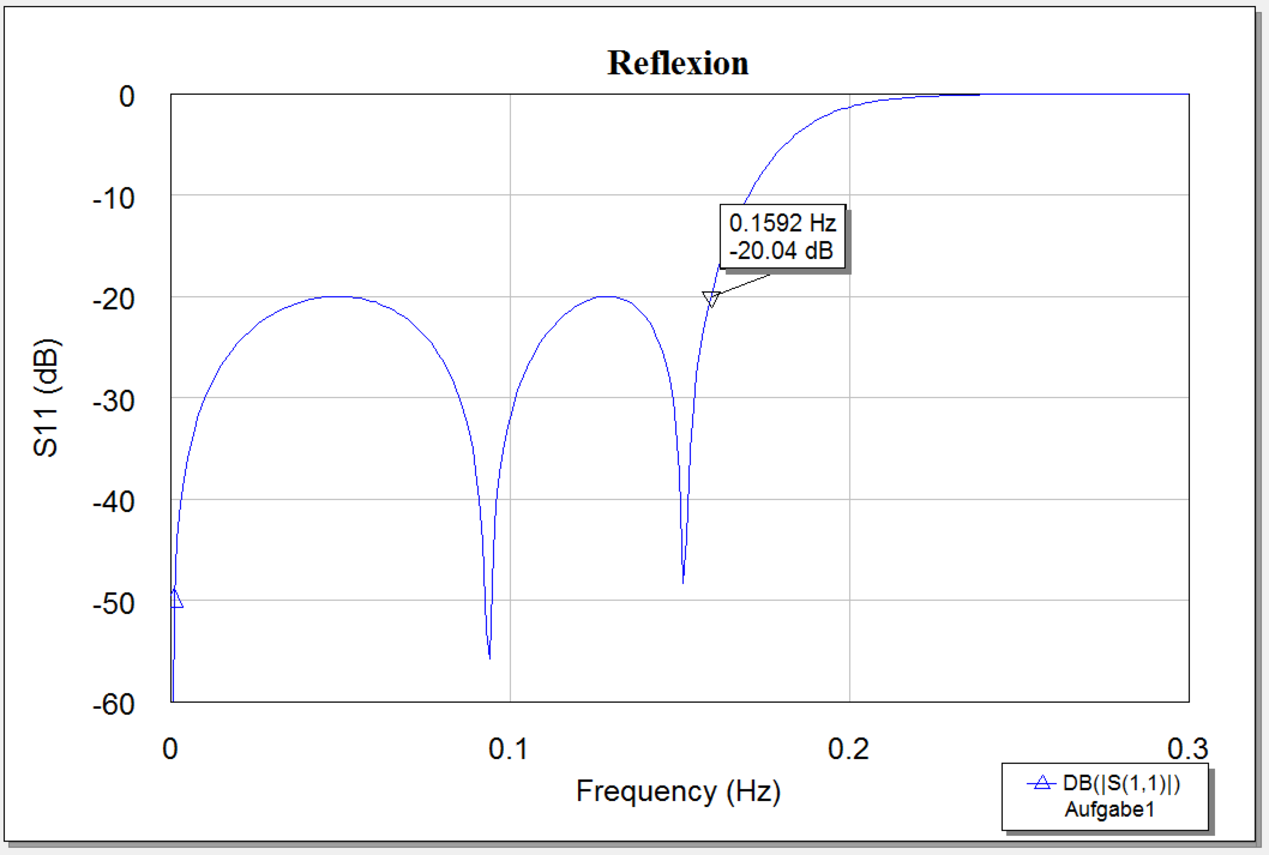
\includegraphics[width=\imagewidth]{images/Prototyp_Reflexion.png}
 	\caption{Reflexion in Passband}
 	\label{fig:Prototyp_Reflexion}
\end{figure}

Zusammenfassend handelt sich beim zu realisierenden Stubfilter um ein Chebyshev Filter 5. Ordnung des Typ 1 mit folgenden Eigeschaften: 
\begin{mdframed}
\begin{equation*} 
\begin{array}{cllll} 
f_C & = & 0.8 GHz \\ 
f_\frac{\lambda}{4} & = & 2 GHz \\ 
l & = & 37.5mm \\
Equirippel (Passband) & = & -0.004355 dB \\
Reflexion (Passband) & = & -20 dB \\
\end{array} 
\end{equation*} 
\end{mdframed}



